\documentclass[12 pt]{article} %Sets the default text size to 11pt and class to article.
%------------------------Dimensions--------------------------------------------
\topmargin=0.0in %length of margin at the top of the page (1 inch added by default)
\oddsidemargin=0.0in %length of margin on sides for odd pages
\evensidemargin=0in %length of margin on sides for even pages
\textwidth=6.5in %How wide you want your text to be
\marginparwidth=0.5in
\headheight=0pt %1in margins at top and bottom (1 inch is added to this value by default)
\headsep=0pt %Increase to increase white space in between headers and the top of the page
\textheight=9.0in %How tall the text body is allowed to be on each page
\setlength\parindent{0pt} % Removes all indentation from paragraphs

% \usepackage[T1]{fontenc}
% \usepackage{textcomp}
% \renewcommand{\familydefault}{\sfdefault}

\usepackage{times}
\usepackage{floatrow}
\usepackage{tgpagella}
\usepackage{lmodern}
\usepackage{fancyvrb}
\usepackage{color}
\usepackage{lipsum}
\usepackage{wrapfig}
\usepackage[utf8]{inputenc}
\usepackage{array, xcolor}
\usepackage{graphicx}
\usepackage{fancyhdr}
\pagestyle{fancy}
\renewcommand{\headrulewidth}{0pt}
\fancyhead{}
\makeatletter
\def\PY@reset{\let\PY@it=\relax \let\PY@bf=\relax%
    \let\PY@ul=\relax \let\PY@tc=\relax%
    \let\PY@bc=\relax \let\PY@ff=\relax}
\def\PY@tok#1{\csname PY@tok@#1\endcsname}
\def\PY@toks#1+{\ifx\relax#1\empty\else%
    \PY@tok{#1}\expandafter\PY@toks\fi}
\def\PY@do#1{\PY@bc{\PY@tc{\PY@ul{%
    \PY@it{\PY@bf{\PY@ff{#1}}}}}}}
\def\PY#1#2{\PY@reset\PY@toks#1+\relax+\PY@do{#2}}

\expandafter\def\csname PY@tok@gd\endcsname{\def\PY@tc##1{\textcolor[rgb]{0.63,0.00,0.00}{##1}}}
\expandafter\def\csname PY@tok@gu\endcsname{\let\PY@bf=\textbf\def\PY@tc##1{\textcolor[rgb]{0.50,0.00,0.50}{##1}}}
\expandafter\def\csname PY@tok@gt\endcsname{\def\PY@tc##1{\textcolor[rgb]{0.00,0.27,0.87}{##1}}}
\expandafter\def\csname PY@tok@gs\endcsname{\let\PY@bf=\textbf}
\expandafter\def\csname PY@tok@gr\endcsname{\def\PY@tc##1{\textcolor[rgb]{1.00,0.00,0.00}{##1}}}
\expandafter\def\csname PY@tok@cm\endcsname{\let\PY@it=\textit\def\PY@tc##1{\textcolor[rgb]{0.25,0.50,0.50}{##1}}}
\expandafter\def\csname PY@tok@vg\endcsname{\def\PY@tc##1{\textcolor[rgb]{0.10,0.09,0.49}{##1}}}
\expandafter\def\csname PY@tok@m\endcsname{\def\PY@tc##1{\textcolor[rgb]{0.40,0.40,0.40}{##1}}}
\expandafter\def\csname PY@tok@mh\endcsname{\def\PY@tc##1{\textcolor[rgb]{0.40,0.40,0.40}{##1}}}
\expandafter\def\csname PY@tok@go\endcsname{\def\PY@tc##1{\textcolor[rgb]{0.53,0.53,0.53}{##1}}}
\expandafter\def\csname PY@tok@ge\endcsname{\let\PY@it=\textit}
\expandafter\def\csname PY@tok@vc\endcsname{\def\PY@tc##1{\textcolor[rgb]{0.10,0.09,0.49}{##1}}}
\expandafter\def\csname PY@tok@il\endcsname{\def\PY@tc##1{\textcolor[rgb]{0.40,0.40,0.40}{##1}}}
\expandafter\def\csname PY@tok@cs\endcsname{\let\PY@it=\textit\def\PY@tc##1{\textcolor[rgb]{0.25,0.50,0.50}{##1}}}
\expandafter\def\csname PY@tok@cp\endcsname{\def\PY@tc##1{\textcolor[rgb]{0.74,0.48,0.00}{##1}}}
\expandafter\def\csname PY@tok@gi\endcsname{\def\PY@tc##1{\textcolor[rgb]{0.00,0.63,0.00}{##1}}}
\expandafter\def\csname PY@tok@gh\endcsname{\let\PY@bf=\textbf\def\PY@tc##1{\textcolor[rgb]{0.00,0.00,0.50}{##1}}}
\expandafter\def\csname PY@tok@ni\endcsname{\let\PY@bf=\textbf\def\PY@tc##1{\textcolor[rgb]{0.60,0.60,0.60}{##1}}}
\expandafter\def\csname PY@tok@nl\endcsname{\def\PY@tc##1{\textcolor[rgb]{0.63,0.63,0.00}{##1}}}
\expandafter\def\csname PY@tok@nn\endcsname{\let\PY@bf=\textbf\def\PY@tc##1{\textcolor[rgb]{0.00,0.00,1.00}{##1}}}
\expandafter\def\csname PY@tok@no\endcsname{\def\PY@tc##1{\textcolor[rgb]{0.53,0.00,0.00}{##1}}}
\expandafter\def\csname PY@tok@na\endcsname{\def\PY@tc##1{\textcolor[rgb]{0.49,0.56,0.16}{##1}}}
\expandafter\def\csname PY@tok@nb\endcsname{\def\PY@tc##1{\textcolor[rgb]{0.00,0.50,0.00}{##1}}}
\expandafter\def\csname PY@tok@nc\endcsname{\let\PY@bf=\textbf\def\PY@tc##1{\textcolor[rgb]{0.00,0.00,1.00}{##1}}}
\expandafter\def\csname PY@tok@nd\endcsname{\def\PY@tc##1{\textcolor[rgb]{0.67,0.13,1.00}{##1}}}
\expandafter\def\csname PY@tok@ne\endcsname{\let\PY@bf=\textbf\def\PY@tc##1{\textcolor[rgb]{0.82,0.25,0.23}{##1}}}
\expandafter\def\csname PY@tok@nf\endcsname{\def\PY@tc##1{\textcolor[rgb]{0.00,0.00,1.00}{##1}}}
\expandafter\def\csname PY@tok@si\endcsname{\let\PY@bf=\textbf\def\PY@tc##1{\textcolor[rgb]{0.73,0.40,0.53}{##1}}}
\expandafter\def\csname PY@tok@s2\endcsname{\def\PY@tc##1{\textcolor[rgb]{0.73,0.13,0.13}{##1}}}
\expandafter\def\csname PY@tok@vi\endcsname{\def\PY@tc##1{\textcolor[rgb]{0.10,0.09,0.49}{##1}}}
\expandafter\def\csname PY@tok@nt\endcsname{\let\PY@bf=\textbf\def\PY@tc##1{\textcolor[rgb]{0.00,0.50,0.00}{##1}}}
\expandafter\def\csname PY@tok@nv\endcsname{\def\PY@tc##1{\textcolor[rgb]{0.10,0.09,0.49}{##1}}}
\expandafter\def\csname PY@tok@s1\endcsname{\def\PY@tc##1{\textcolor[rgb]{0.73,0.13,0.13}{##1}}}
\expandafter\def\csname PY@tok@sh\endcsname{\def\PY@tc##1{\textcolor[rgb]{0.73,0.13,0.13}{##1}}}
\expandafter\def\csname PY@tok@sc\endcsname{\def\PY@tc##1{\textcolor[rgb]{0.73,0.13,0.13}{##1}}}
\expandafter\def\csname PY@tok@sx\endcsname{\def\PY@tc##1{\textcolor[rgb]{0.00,0.50,0.00}{##1}}}
\expandafter\def\csname PY@tok@bp\endcsname{\def\PY@tc##1{\textcolor[rgb]{0.00,0.50,0.00}{##1}}}
\expandafter\def\csname PY@tok@c1\endcsname{\let\PY@it=\textit\def\PY@tc##1{\textcolor[rgb]{0.25,0.50,0.50}{##1}}}
\expandafter\def\csname PY@tok@kc\endcsname{\let\PY@bf=\textbf\def\PY@tc##1{\textcolor[rgb]{0.00,0.50,0.00}{##1}}}
\expandafter\def\csname PY@tok@c\endcsname{\let\PY@it=\textit\def\PY@tc##1{\textcolor[rgb]{0.25,0.50,0.50}{##1}}}
\expandafter\def\csname PY@tok@mf\endcsname{\def\PY@tc##1{\textcolor[rgb]{0.40,0.40,0.40}{##1}}}
\expandafter\def\csname PY@tok@err\endcsname{\def\PY@bc##1{\setlength{\fboxsep}{0pt}\fcolorbox[rgb]{1.00,0.00,0.00}{1,1,1}{\strut ##1}}}
\expandafter\def\csname PY@tok@kd\endcsname{\let\PY@bf=\textbf\def\PY@tc##1{\textcolor[rgb]{0.00,0.50,0.00}{##1}}}
\expandafter\def\csname PY@tok@ss\endcsname{\def\PY@tc##1{\textcolor[rgb]{0.10,0.09,0.49}{##1}}}
\expandafter\def\csname PY@tok@sr\endcsname{\def\PY@tc##1{\textcolor[rgb]{0.73,0.40,0.53}{##1}}}
\expandafter\def\csname PY@tok@mo\endcsname{\def\PY@tc##1{\textcolor[rgb]{0.40,0.40,0.40}{##1}}}
\expandafter\def\csname PY@tok@kn\endcsname{\let\PY@bf=\textbf\def\PY@tc##1{\textcolor[rgb]{0.00,0.50,0.00}{##1}}}
\expandafter\def\csname PY@tok@mi\endcsname{\def\PY@tc##1{\textcolor[rgb]{0.40,0.40,0.40}{##1}}}
\expandafter\def\csname PY@tok@gp\endcsname{\let\PY@bf=\textbf\def\PY@tc##1{\textcolor[rgb]{0.00,0.00,0.50}{##1}}}
\expandafter\def\csname PY@tok@o\endcsname{\def\PY@tc##1{\textcolor[rgb]{0.40,0.40,0.40}{##1}}}
\expandafter\def\csname PY@tok@kr\endcsname{\let\PY@bf=\textbf\def\PY@tc##1{\textcolor[rgb]{0.00,0.50,0.00}{##1}}}
\expandafter\def\csname PY@tok@s\endcsname{\def\PY@tc##1{\textcolor[rgb]{0.73,0.13,0.13}{##1}}}
\expandafter\def\csname PY@tok@kp\endcsname{\def\PY@tc##1{\textcolor[rgb]{0.00,0.50,0.00}{##1}}}
\expandafter\def\csname PY@tok@w\endcsname{\def\PY@tc##1{\textcolor[rgb]{0.73,0.73,0.73}{##1}}}
\expandafter\def\csname PY@tok@kt\endcsname{\def\PY@tc##1{\textcolor[rgb]{0.69,0.00,0.25}{##1}}}
\expandafter\def\csname PY@tok@ow\endcsname{\let\PY@bf=\textbf\def\PY@tc##1{\textcolor[rgb]{0.67,0.13,1.00}{##1}}}
\expandafter\def\csname PY@tok@sb\endcsname{\def\PY@tc##1{\textcolor[rgb]{0.73,0.13,0.13}{##1}}}
\expandafter\def\csname PY@tok@k\endcsname{\let\PY@bf=\textbf\def\PY@tc##1{\textcolor[rgb]{0.00,0.50,0.00}{##1}}}
\expandafter\def\csname PY@tok@se\endcsname{\let\PY@bf=\textbf\def\PY@tc##1{\textcolor[rgb]{0.73,0.40,0.13}{##1}}}
\expandafter\def\csname PY@tok@sd\endcsname{\let\PY@it=\textit\def\PY@tc##1{\textcolor[rgb]{0.73,0.13,0.13}{##1}}}

\def\PYZbs{\char`\\}
\def\PYZus{\char`\_}
\def\PYZob{\char`\{}
\def\PYZcb{\char`\}}
\def\PYZca{\char`\^}
\def\PYZam{\char`\&}
\def\PYZlt{\char`\<}
\def\PYZgt{\char`\>}
\def\PYZsh{\char`\#}
\def\PYZpc{\char`\%}
\def\PYZdl{\char`\$}
\def\PYZhy{\char`\-}
\def\PYZsq{\char`\'}
\def\PYZdq{\char`\"}
\def\PYZti{\char`\~}
% for compatibility with earlier versions
\def\PYZat{@}
\def\PYZlb{[}
\def\PYZrb{]}
\makeatother

% pygmentize -f latex function.java > output.tex

\usepackage[hidelinks]{hyperref}
\usepackage{framed}
\usepackage{tikz}

\definecolor{dark-red}{rgb}{0.4,0.15,0.15}
\definecolor{dark-blue}{rgb}{0.15,0.15,0.4}
\definecolor{medium-blue}{rgb}{0,0,0.5}
\hypersetup{
    colorlinks, linkcolor={dark-red},
    citecolor={dark-blue}, urlcolor={medium-blue}
}


\begin{document}
\title{\vskip -5em \bf Near optimal A* path finding}   % type title between braces
\author{
	Andreas Valter, andva287@student.liu.se
}
\date{\today}    % type date between braces
\maketitle
\section{Abstract}
\section{Introduction}
Path finding is the extraction of the shortest route between two points and is mostly a core feature that is needed to control agents in the game. 
With path finding, the user doesn't have to control all elements in the game.
Something that could be boring while playing against an AI or when there is a lot of agents that the user controls at the same time.\\

When developing computer games, each clock cycle is important. This puts a goal for each component in the game engine to be as fast as possible. 
Because when saving computation time on components, it is possible to increase the frame rate or adding more features. \\

Most computer games uses path finding to increase the game quality. For AI agents it makes it possible to go between locations.
For the user, it could make it easier to travel between places.
The most common method of choice is A* to find the shortest path between two points in a map.
The problem with using A* is that it is quite slow, depending on how the map is defined, and a lot of computation is unused in the end.\\

\section{Path finding}
\subsection{A*}
A* is basically a modified Dijkstra algorithm, that is a graph search to find the optimal path between two nodes. 
The search is done using heuristics to find probable next nodes that brings the search closer to the goal. 
For map search, the heuristics is usually the Manhattan distance from the current position to the goal position.
\begin{Verbatim}[commandchars=\\\{\}]
\PY{k}{def} \PY{n+nf}{calculateManhattanDistance}\PY{p}{(}\PY{n+nb+bp}{self}\PY{p}{,} \PY{n}{node}\PY{p}{,} \PY{n}{goal}\PY{p}{)}\PY{p}{:}
    \PY{n}{goalToNode} \PY{o}{=} \PY{n}{nodePos} \PY{o}{\PYZhy{}} \PY{n}{goal}
    \PY{k}{return} \PY{n+nb}{abs}\PY{p}{(}\PY{n}{goalToNode}\PY{o}{.}\PY{n}{x}\PY{p}{)} \PY{o}{+} \PY{n+nb}{abs}\PY{p}{(}\PY{n}{goalToNode}\PY{o}{.}\PY{n}{y}\PY{p}{)}
\end{Verbatim}

This is used to find the most likely next node, in a best-first fashion.
Figure \ref{fig:astarcat} show an example of how the algorithm works.
By adding new nodes as we traverse the map, new nodes to evaluate is added until the solution is found or until the list of nodes to evaluate is empty.
If the list of nodes is empty before a solution is found, we know that it is impossible to find a path between the start and the goal nodes.
As it show, the overhead when calculating is quite small, and this is mostly the case when using A*.
But the worst case when using it is that we are tricked to evaluate a lot of extra positions.
\begin{figure}
	\ffigbox[1.2\FBwidth]
	{\caption{A* algorithm example with a cat trying to find a bone. The values represent distance to cat, distance to bone and total sum.}}
	{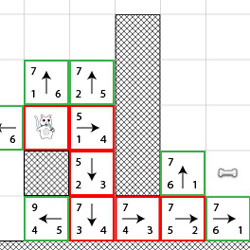
\includegraphics[width=0.39\textwidth]{fig/astarcat.jpg}}
	\label{fig:astarcat}
\end{figure}
At the same time, the A* is calculated under runtime, with the possibility that the path is changed before the goal is reached.
But we still need to find the whole path between the nodes because that is the only way to know which way to start walking.
So a solution where we can calculate the approximate path, with high local quality would be optimal.\\

The solution generated by the A* algorithm is not only correct, but it is also found quite fast. 
\subsection{Near optimal A*}
The {\it Near optimal A*} algorithm tries to solve this problem in a clever way.
By creating a simple definition of the map beforehand, and using that representation to do fast searches, it is possible to save a lot of time.
The simple map consists of a graph structure that represents possible paths trough the map.\\
\begin{figure}	
	\ffigbox[1.2\FBwidth]
	{\caption{Map with start and goal placed.}}
	{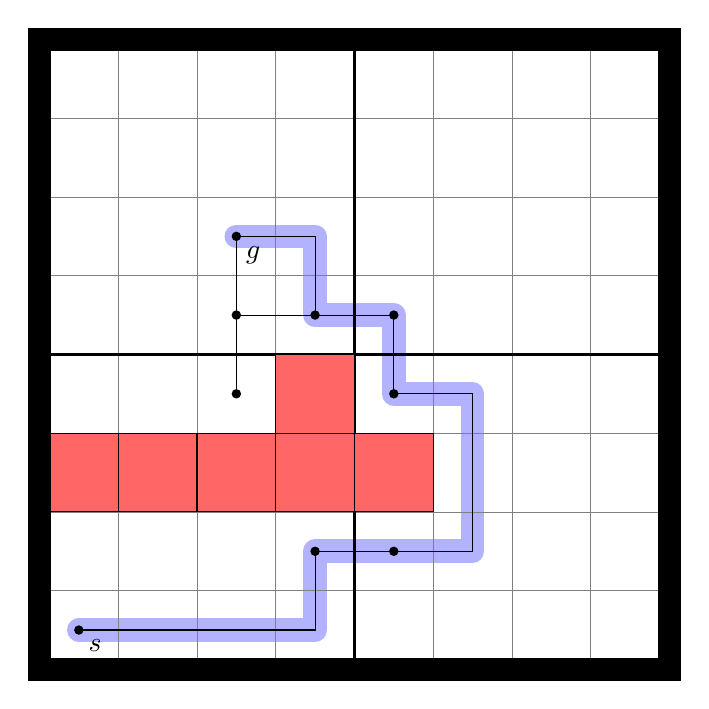
\begin{tikzpicture}
[
	bline/.style={line width=0.3cm,cap=round,join=round, color=blue!30},
	obst/.style={fill=red!60},
	myNodeLine/.style={thin,color=black!100}
]

\def\square{rectangle +(1,1)}
\def\entranceNode{circle (0.06cm)}
% Draw path
% Final path
\draw[bline] (0.5,0.5)--(3.5,0.5)--(3.5,1.5)--(5.5, 1.5)--(5.5, 3.5)--(4.5, 3.5)--(4.5, 4.5)--(3.5,4.5)--(3.5, 5.5)--(2.5,5.5);

% Draw grid 	
\draw[help lines] (0,0) grid (8,8);

% Create cluster lines
\draw[thick] (0,4)--(8,4);
\draw[thick] (4,0)--(4,8);

% Draw obstacle
\draw[obst] (2, 2) \square (3, 2) \square  (3, 3) \square  (4, 2) \square  (1, 2) \square (0, 2) \square;

% Draw border
\draw[line width=0.3cm] (0,0) rectangle +(8,8);

% Draw nodes
\draw[below right] (0.5, 0.5) node(s){$s$};
\draw[below right] (2.5, 5.5) node(t){$g$};
\fill (0.5,0.5) circle (0.06cm) (2.5,5.5) circle (0.06cm);

% Draw lines between nodes
\draw[myNodeLine](2.5, 3.5)--(2.5, 4.5) 
										(3.5, 4.5)--(4.5, 4.5) 
										(3.5, 1.5)--(4.5, 1.5);
										(4.5, 3.5)--(4.5, 4.5);

% Draw intra cluster edges
\draw[myNodeLine](4.5, 1.5)--(5.5, 1.5)--(5.5, 3.5)--(4.5, 3.5)--(4.5, 4.5)--(2.5,4.5);

% Draw connections to start and goal
\draw[myNodeLine](0.5, 0.5)--(3.5, 0.5)--(3.5, 1.5) (2.5, 5.5)--(2.5, 4.5) (2.5,5.5)--(3.5, 5.5)--(3.5, 4.5);

% Create entrance nodes
\fill (4.5,1.5) \entranceNode (3.5, 1.5) \entranceNode;
\fill (3.5, 4.5) \entranceNode (4.5, 3.5) \entranceNode;
\fill (4.5, 4.5) \entranceNode;
\fill (2.5, 4.5) \entranceNode (2.5, 3.5) \entranceNode;

\end{tikzpicture}}
	\label{fig:astarcat}
\end{figure}
The algorithm is done in a couple of steps:\\

Firstly the map is divided into a set of clusters, with a pre specified width.
For each pair of neighbours we locate entrances, defined as points where it is possible to travel from one of the clusters to the other.
If the length of the opening between the two clusters is below a threshold, one entrance is added in the middle, if higher, two entrances are created at the edges.
All entrances are added as nodes into a graph.\\

A* is then used locally to calculate the path between all local entrances in each cluster. 
This creates a graph consisting of a lower representation of the map and possible paths between all clusters.
By temporarily adding the start and goal position to the graph, the correct path can be found by checking the path, without any need to do the costly A*.
To find the optimal path between the start and goal, we use A* again to calculate the path between them.
The difference is that we are only calculating the A* solution between two nodes in the path found in the graph.
This is more optimal because we can calculate sub steps of the path, steps that is further away is not that important so we spend time on refining the close path, knowing that we are walking in the right way.

\end{document}

